\documentclass[1p]{elsarticle_modified}
%\bibliographystyle{elsarticle-num}

%\usepackage[colorlinks]{hyperref}
%\usepackage{abbrmath_seonhwa} %\Abb, \Ascr, \Acal ,\Abf, \Afrak
\usepackage{amsfonts}
\usepackage{amssymb}
\usepackage{amsmath}
\usepackage{amsthm}
\usepackage{scalefnt}
\usepackage{amsbsy}
\usepackage{kotex}
\usepackage{caption}
\usepackage{subfig}
\usepackage{color}
\usepackage{graphicx}
\usepackage{xcolor} %% white, black, red, green, blue, cyan, magenta, yellow
\usepackage{float}
\usepackage{setspace}
\usepackage{hyperref}

\usepackage{tikz}
\usetikzlibrary{arrows}

\usepackage{multirow}
\usepackage{array} % fixed length table
\usepackage{hhline}

%%%%%%%%%%%%%%%%%%%%%
\makeatletter
\renewcommand*\env@matrix[1][\arraystretch]{%
	\edef\arraystretch{#1}%
	\hskip -\arraycolsep
	\let\@ifnextchar\new@ifnextchar
	\array{*\c@MaxMatrixCols c}}
\makeatother %https://tex.stackexchange.com/questions/14071/how-can-i-increase-the-line-spacing-in-a-matrix
%%%%%%%%%%%%%%%

\usepackage[normalem]{ulem}

\newcommand{\msout}[1]{\ifmmode\text{\sout{\ensuremath{#1}}}\else\sout{#1}\fi}
%SOURCE: \msout is \stkout macro in https://tex.stackexchange.com/questions/20609/strikeout-in-math-mode

\newcommand{\cancel}[1]{
	\ifmmode
	{\color{red}\msout{#1}}
	\else
	{\color{red}\sout{#1}}
	\fi
}

\newcommand{\add}[1]{
	{\color{blue}\uwave{#1}}
}

\newcommand{\replace}[2]{
	\ifmmode
	{\color{red}\msout{#1}}{\color{blue}\uwave{#2}}
	\else
	{\color{red}\sout{#1}}{\color{blue}\uwave{#2}}
	\fi
}

\newcommand{\Sol}{\mathcal{S}} %segment
\newcommand{\D}{D} %diagram
\newcommand{\A}{\mathcal{A}} %arc


%%%%%%%%%%%%%%%%%%%%%%%%%%%%%5 test

\def\sl{\operatorname{\textup{SL}}(2,\Cbb)}
\def\psl{\operatorname{\textup{PSL}}(2,\Cbb)}
\def\quan{\mkern 1mu \triangleright \mkern 1mu}

\theoremstyle{definition}
\newtheorem{thm}{Theorem}[section]
\newtheorem{prop}[thm]{Proposition}
\newtheorem{lem}[thm]{Lemma}
\newtheorem{ques}[thm]{Question}
\newtheorem{cor}[thm]{Corollary}
\newtheorem{defn}[thm]{Definition}
\newtheorem{exam}[thm]{Example}
\newtheorem{rmk}[thm]{Remark}
\newtheorem{alg}[thm]{Algorithm}

\newcommand{\I}{\sqrt{-1}}
\begin{document}

%\begin{frontmatter}
%
%\title{Boundary parabolic representations of knots up to 8 crossings}
%
%%% Group authors per affiliation:
%\author{Yunhi Cho} 
%\address{Department of Mathematics, University of Seoul, Seoul, Korea}
%\ead{yhcho@uos.ac.kr}
%
%
%\author{Seonhwa Kim} %\fnref{s_kim}}
%\address{Center for Geometry and Physics, Institute for Basic Science, Pohang, 37673, Korea}
%\ead{ryeona17@ibs.re.kr}
%
%\author{Hyuk Kim}
%\address{Department of Mathematical Sciences, Seoul National University, Seoul 08826, Korea}
%\ead{hyukkim@snu.ac.kr}
%
%\author{Seokbeom Yoon}
%\address{Department of Mathematical Sciences, Seoul National University, Seoul, 08826,  Korea}
%\ead{sbyoon15@snu.ac.kr}
%
%\begin{abstract}
%We find all boundary parabolic representation of knots up to 8 crossings.
%
%\end{abstract}
%\begin{keyword}
%    \MSC[2010] 57M25 
%\end{keyword}
%
%\end{frontmatter}

%\linenumbers
%\tableofcontents
%
\newcommand\colored[1]{\textcolor{white}{\rule[-0.35ex]{0.8em}{1.4ex}}\kern-0.8em\color{red} #1}%
%\newcommand\colored[1]{\textcolor{white}{ #1}\kern-2.17ex	\textcolor{white}{ #1}\kern-1.81ex	\textcolor{white}{ #1}\kern-2.15ex\color{red}#1	}

{\Large $\underline{12n_{0745}~(K12n_{0745})}$}

\setlength{\tabcolsep}{10pt}
\renewcommand{\arraystretch}{1.6}
\vspace{1cm}\begin{tabular}{m{100pt}>{\centering\arraybackslash}m{274pt}}
\multirow{5}{120pt}{
	\centering
	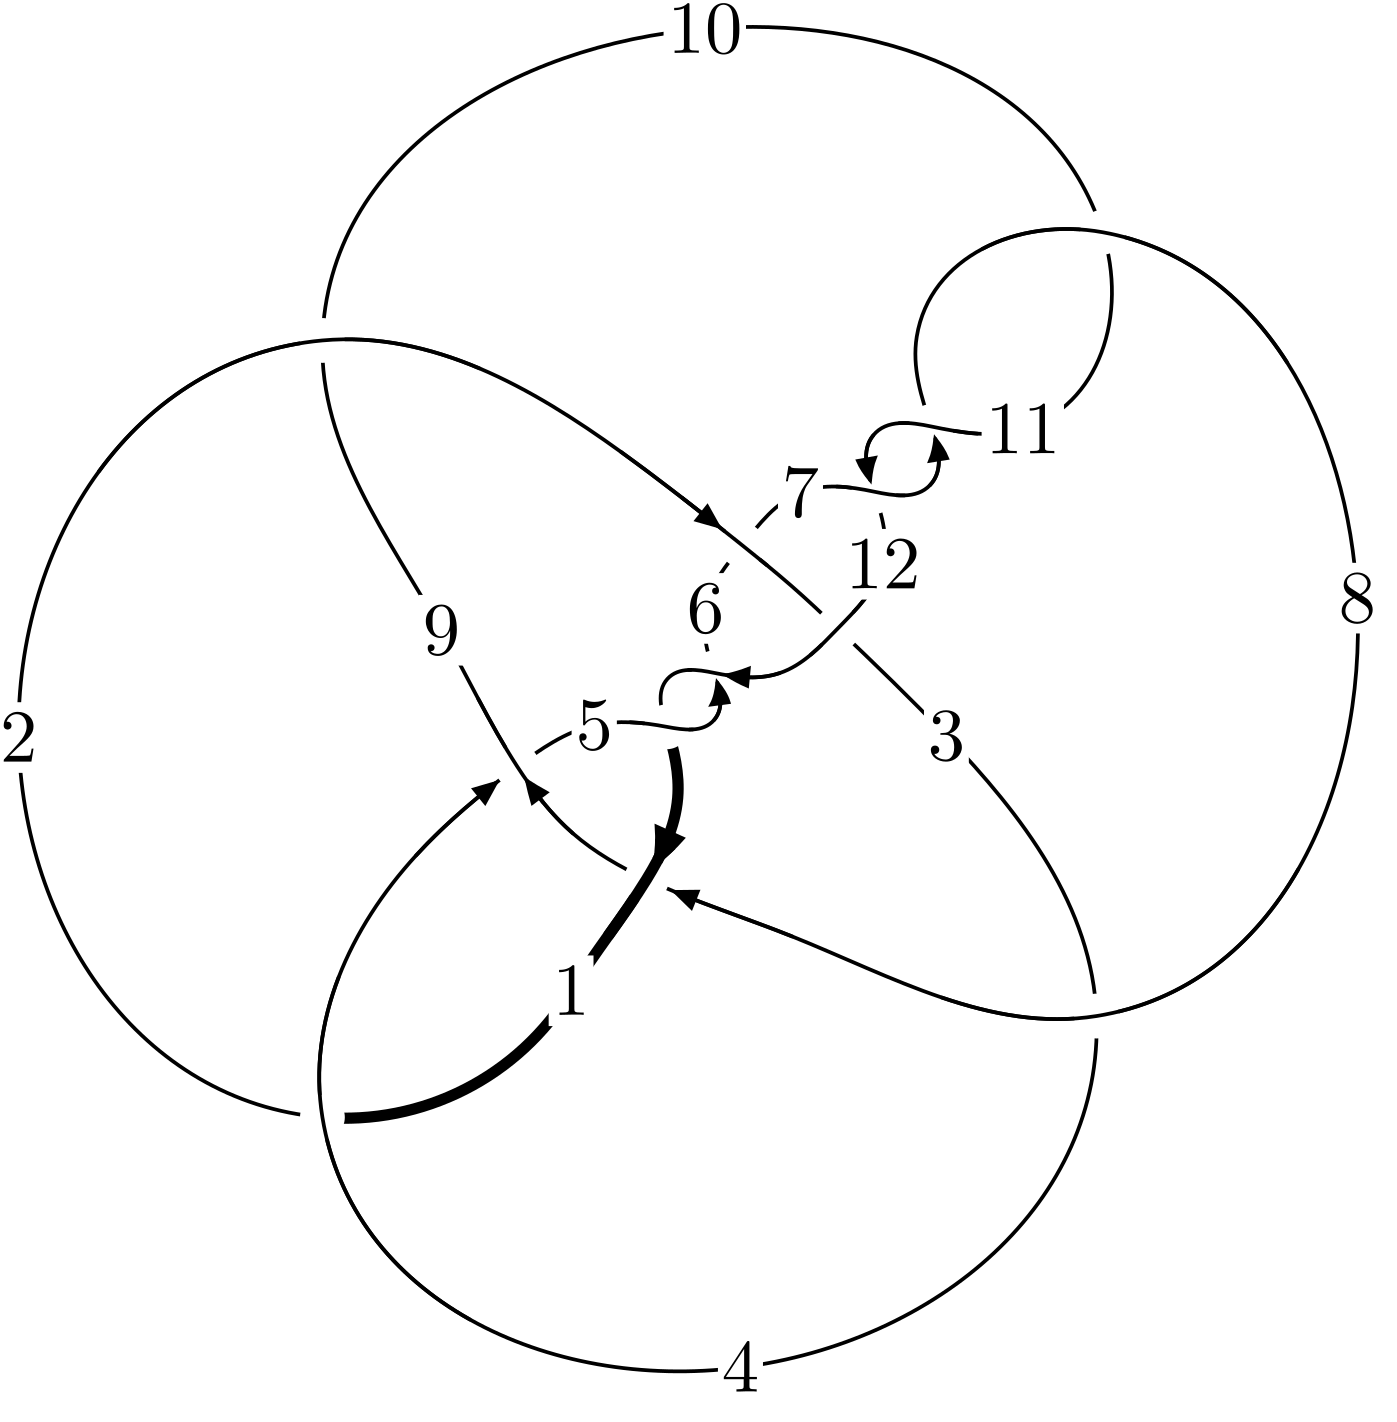
\includegraphics[width=112pt]{../../../GIT/diagram.site/Diagrams/png/2834_12n_0745.png}\\
\ \ \ A knot diagram\footnotemark}&
\allowdisplaybreaks
\textbf{Linearized knot diagam} \\
\cline{2-2}
 &
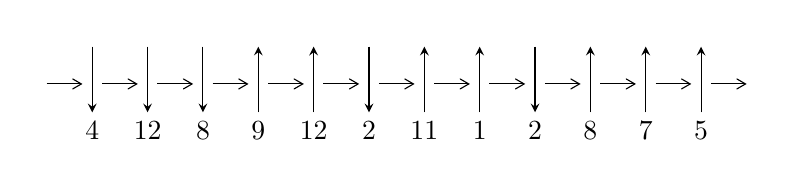
\begin{tikzpicture}[x=20pt, y=17pt]
	% nodes
	\node (C0) at (0, 0) {};
	\node (C1) at (1, 0) {};
	\node (C1U) at (1, +1) {};
	\node (C1D) at (1, -1) {4};

	\node (C2) at (2, 0) {};
	\node (C2U) at (2, +1) {};
	\node (C2D) at (2, -1) {12};

	\node (C3) at (3, 0) {};
	\node (C3U) at (3, +1) {};
	\node (C3D) at (3, -1) {8};

	\node (C4) at (4, 0) {};
	\node (C4U) at (4, +1) {};
	\node (C4D) at (4, -1) {9};

	\node (C5) at (5, 0) {};
	\node (C5U) at (5, +1) {};
	\node (C5D) at (5, -1) {12};

	\node (C6) at (6, 0) {};
	\node (C6U) at (6, +1) {};
	\node (C6D) at (6, -1) {2};

	\node (C7) at (7, 0) {};
	\node (C7U) at (7, +1) {};
	\node (C7D) at (7, -1) {11};

	\node (C8) at (8, 0) {};
	\node (C8U) at (8, +1) {};
	\node (C8D) at (8, -1) {1};

	\node (C9) at (9, 0) {};
	\node (C9U) at (9, +1) {};
	\node (C9D) at (9, -1) {2};

	\node (C10) at (10, 0) {};
	\node (C10U) at (10, +1) {};
	\node (C10D) at (10, -1) {8};

	\node (C11) at (11, 0) {};
	\node (C11U) at (11, +1) {};
	\node (C11D) at (11, -1) {7};

	\node (C12) at (12, 0) {};
	\node (C12U) at (12, +1) {};
	\node (C12D) at (12, -1) {5};
	\node (C13) at (13, 0) {};

	% arrows
	\draw[->,>={angle 60}]
	(C0) edge (C1) (C1) edge (C2) (C2) edge (C3) (C3) edge (C4) (C4) edge (C5) (C5) edge (C6) (C6) edge (C7) (C7) edge (C8) (C8) edge (C9) (C9) edge (C10) (C10) edge (C11) (C11) edge (C12) (C12) edge (C13) ;	\draw[->,>=stealth]
	(C1U) edge (C1D) (C2U) edge (C2D) (C3U) edge (C3D) (C4D) edge (C4U) (C5D) edge (C5U) (C6U) edge (C6D) (C7D) edge (C7U) (C8D) edge (C8U) (C9U) edge (C9D) (C10D) edge (C10U) (C11D) edge (C11U) (C12D) edge (C12U) ;
	\end{tikzpicture} \\
\hhline{~~} \\& 
\textbf{Solving Sequence} \\ \cline{2-2} 
 &
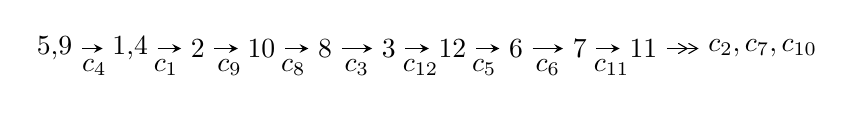
\begin{tikzpicture}[x=23pt, y=7pt]
	% node
	\node (A0) at (-1/8, 0) {5,9};
	\node (A1) at (17/16, 0) {1,4};
	\node (A2) at (17/8, 0) {2};
	\node (A3) at (25/8, 0) {10};
	\node (A4) at (33/8, 0) {8};
	\node (A5) at (41/8, 0) {3};
	\node (A6) at (49/8, 0) {12};
	\node (A7) at (57/8, 0) {6};
	\node (A8) at (65/8, 0) {7};
	\node (A9) at (73/8, 0) {11};
	\node (C1) at (1/2, -1) {$c_{4}$};
	\node (C2) at (13/8, -1) {$c_{1}$};
	\node (C3) at (21/8, -1) {$c_{9}$};
	\node (C4) at (29/8, -1) {$c_{8}$};
	\node (C5) at (37/8, -1) {$c_{3}$};
	\node (C6) at (45/8, -1) {$c_{12}$};
	\node (C7) at (53/8, -1) {$c_{5}$};
	\node (C8) at (61/8, -1) {$c_{6}$};
	\node (C9) at (69/8, -1) {$c_{11}$};
	\node (A10) at (11, 0) {$c_{2},c_{7},c_{10}$};

	% edge
	\draw[->,>=stealth]	
	(A0) edge (A1) (A1) edge (A2) (A2) edge (A3) (A3) edge (A4) (A4) edge (A5) (A5) edge (A6) (A6) edge (A7) (A7) edge (A8) (A8) edge (A9) ;
	\draw[->>,>={angle 60}]	
	(A9) edge (A10);
\end{tikzpicture} \\ 

\end{tabular} \\

\footnotetext{
The image of knot diagram is generated by the software ``\textbf{Draw programme}" developed by Andrew Bartholomew(\url{http://www.layer8.co.uk/maths/draw/index.htm\#Running-draw}), where we modified some parts for our purpose(\url{https://github.com/CATsTAILs/LinksPainter}).
}\phantom \\ \newline 
\centering \textbf{Ideals for irreducible components\footnotemark of $X_{\text{par}}$} 
 
\begin{align*}
I^u_{1}&=\langle 
-7.72392\times10^{20} u^{31}-1.85563\times10^{20} u^{30}+\cdots+1.12162\times10^{21} b+1.59649\times10^{21},\;a-1,\\
\phantom{I^u_{1}}&\phantom{= \langle  }u^{32}- u^{30}+\cdots-2 u+1\rangle \\
I^u_{2}&=\langle 
-1.04878\times10^{64} u^{47}-4.13535\times10^{64} u^{46}+\cdots+4.36700\times10^{65} b+2.54209\times10^{65},\\
\phantom{I^u_{2}}&\phantom{= \langle  }-6.42157\times10^{113} u^{47}-2.04396\times10^{114} u^{46}+\cdots+2.06184\times10^{114} a-4.26495\times10^{114},\\
\phantom{I^u_{2}}&\phantom{= \langle  }u^{48}+3 u^{47}+\cdots-8 u+4\rangle \\
I^u_{3}&=\langle 
-4169 u^{17}-110 u^{16}+\cdots+1711 b+2133,\;a+1,\;u^{18}+4 u^{16}+\cdots- u+1\rangle \\
\\
\end{align*}
\raggedright * 3 irreducible components of $\dim_{\mathbb{C}}=0$, with total 98 representations.\\
\footnotetext{All coefficients of polynomials are rational numbers. But the coefficients are sometimes approximated in decimal forms when there is not enough margin.}
\newpage
\renewcommand{\arraystretch}{1}
\centering \section*{I. $I^u_{1}= \langle -7.72\times10^{20} u^{31}-1.86\times10^{20} u^{30}+\cdots+1.12\times10^{21} b+1.60\times10^{21},\;a-1,\;u^{32}- u^{30}+\cdots-2 u+1 \rangle$}
\flushleft \textbf{(i) Arc colorings}\\
\begin{tabular}{m{7pt} m{180pt} m{7pt} m{180pt} }
\flushright $a_{5}=$&$\begin{pmatrix}1\\0\end{pmatrix}$ \\
\flushright $a_{9}=$&$\begin{pmatrix}0\\u\end{pmatrix}$ \\
\flushright $a_{1}=$&$\begin{pmatrix}1\\0.688642 u^{31}+0.165443 u^{30}+\cdots+2.18437 u-1.42339\end{pmatrix}$ \\
\flushright $a_{4}=$&$\begin{pmatrix}1\\u^2\end{pmatrix}$ \\
\flushright $a_{2}=$&$\begin{pmatrix}-0.688642 u^{31}-0.165443 u^{30}+\cdots-2.18437 u+2.42339\\0.608785 u^{31}+0.235945 u^{30}+\cdots+2.54213 u-1.25794\end{pmatrix}$ \\
\flushright $a_{10}=$&$\begin{pmatrix}0.678532 u^{31}+0.284449 u^{30}+\cdots+1.99493 u-1.92526\\-0.695736 u^{31}-0.103896 u^{30}+\cdots-2.15066 u+0.952167\end{pmatrix}$ \\
\flushright $a_{8}=$&$\begin{pmatrix}- u\\-0.165443 u^{31}-0.0798571 u^{30}+\cdots+1.04610 u+0.688642\end{pmatrix}$ \\
\flushright $a_{3}=$&$\begin{pmatrix}-0.0798571 u^{31}+0.0705021 u^{30}+\cdots+0.357757 u+1.16544\\0.220463 u^{31}-0.127057 u^{30}+\cdots-0.347333 u-0.749034\end{pmatrix}$ \\
\flushright $a_{12}=$&$\begin{pmatrix}-0.688642 u^{31}-0.165443 u^{30}+\cdots-2.18437 u+2.42339\\0.688642 u^{31}+0.165443 u^{30}+\cdots+2.18437 u-1.42339\end{pmatrix}$ \\
\flushright $a_{6}=$&$\begin{pmatrix}-1.07690 u^{31}-0.654094 u^{30}+\cdots-8.58223 u+0.101317\\0.388260 u^{31}+0.488651 u^{30}+\cdots+6.39786 u+2.32207\end{pmatrix}$ \\
\flushright $a_{7}=$&$\begin{pmatrix}-0.390513 u^{31}-0.541351 u^{30}+\cdots-6.51468 u-1.02957\\0.00795809 u^{31}+0.188677 u^{30}+\cdots+3.52208 u+2.59118\end{pmatrix}$ \\
\flushright $a_{11}=$&$\begin{pmatrix}0.657110 u^{31}+0.487486 u^{30}+\cdots+2.71903 u-2.58761\\-1.04986 u^{31}-0.281223 u^{30}+\cdots-4.71166 u+1.64877\end{pmatrix}$\\&\end{tabular}
\flushleft \textbf{(ii) Obstruction class $= -1$}\\~\\
\flushleft \textbf{(iii) Cusp Shapes $= -\frac{5229796107208695447003}{1121615042862392489704} u^{31}-\frac{715184273316583329535}{1121615042862392489704} u^{30}+\cdots-\frac{8046640764422946709729}{1121615042862392489704} u+\frac{1349461904188813944858}{140201880357799061213}$}\\~\\
\newpage\renewcommand{\arraystretch}{1}
\flushleft \textbf{(iv) u-Polynomials at the component}\newline \\
\begin{tabular}{m{50pt}|m{274pt}}
Crossings & \hspace{64pt}u-Polynomials at each crossing \\
\hline $$\begin{aligned}c_{1}\end{aligned}$$&$\begin{aligned}
&u^{32}-20 u^{31}+\cdots-30 u+4
\end{aligned}$\\
\hline $$\begin{aligned}c_{2},c_{6}\end{aligned}$$&$\begin{aligned}
&u^{32}+3 u^{31}+\cdots+4 u+1
\end{aligned}$\\
\hline $$\begin{aligned}c_{3},c_{9}\end{aligned}$$&$\begin{aligned}
&u^{32}- u^{31}+\cdots-4 u+1
\end{aligned}$\\
\hline $$\begin{aligned}c_{4},c_{8}\end{aligned}$$&$\begin{aligned}
&u^{32}- u^{30}+\cdots-2 u+1
\end{aligned}$\\
\hline $$\begin{aligned}c_{5},c_{12}\end{aligned}$$&$\begin{aligned}
&u^{32}-22 u^{31}+\cdots-65536 u+4096
\end{aligned}$\\
\hline $$\begin{aligned}c_{7},c_{10},c_{11}\end{aligned}$$&$\begin{aligned}
&u^{32}+9 u^{31}+\cdots+84 u+16
\end{aligned}$\\
\hline
\end{tabular}\\~\\
\newpage\renewcommand{\arraystretch}{1}
\flushleft \textbf{(v) Riley Polynomials at the component}\newline \\
\begin{tabular}{m{50pt}|m{274pt}}
Crossings & \hspace{64pt}Riley Polynomials at each crossing \\
\hline $$\begin{aligned}c_{1}\end{aligned}$$&$\begin{aligned}
&y^{32}+6 y^{31}+\cdots+52 y+16
\end{aligned}$\\
\hline $$\begin{aligned}c_{2},c_{6}\end{aligned}$$&$\begin{aligned}
&y^{32}+31 y^{31}+\cdots+16 y+1
\end{aligned}$\\
\hline $$\begin{aligned}c_{3},c_{9}\end{aligned}$$&$\begin{aligned}
&y^{32}+3 y^{31}+\cdots+28 y+1
\end{aligned}$\\
\hline $$\begin{aligned}c_{4},c_{8}\end{aligned}$$&$\begin{aligned}
&y^{32}-2 y^{31}+\cdots-6 y+1
\end{aligned}$\\
\hline $$\begin{aligned}c_{5},c_{12}\end{aligned}$$&$\begin{aligned}
&y^{32}+20 y^{31}+\cdots-58720256 y+16777216
\end{aligned}$\\
\hline $$\begin{aligned}c_{7},c_{10},c_{11}\end{aligned}$$&$\begin{aligned}
&y^{32}+29 y^{31}+\cdots+976 y+256
\end{aligned}$\\
\hline
\end{tabular}\\~\\
\newpage\flushleft \textbf{(vi) Complex Volumes and Cusp Shapes}
$$\begin{array}{c|c|c}  
\text{Solutions to }I^u_{1}& \I (\text{vol} + \sqrt{-1}CS) & \text{Cusp shape}\\
 \hline 
\begin{aligned}
u &= \phantom{-}0.854141 + 0.589787 I \\
a &= \phantom{-}1.00000\phantom{ +0.000000I} \\
b &= \phantom{-}1.61917 - 0.24070 I\end{aligned}
 & \phantom{-}1.65554 + 9.31216 I & \phantom{-}1.84214 - 8.38213 I \\ \hline\begin{aligned}
u &= \phantom{-}0.854141 - 0.589787 I \\
a &= \phantom{-}1.00000\phantom{ +0.000000I} \\
b &= \phantom{-}1.61917 + 0.24070 I\end{aligned}
 & \phantom{-}1.65554 - 9.31216 I & \phantom{-}1.84214 + 8.38213 I \\ \hline\begin{aligned}
u &= -0.681898 + 0.783221 I \\
a &= \phantom{-}1.00000\phantom{ +0.000000I} \\
b &= \phantom{-}1.05126 - 1.11867 I\end{aligned}
 & -2.14431 - 0.79389 I & -0.82722 + 2.16238 I \\ \hline\begin{aligned}
u &= -0.681898 - 0.783221 I \\
a &= \phantom{-}1.00000\phantom{ +0.000000I} \\
b &= \phantom{-}1.05126 + 1.11867 I\end{aligned}
 & -2.14431 + 0.79389 I & -0.82722 - 2.16238 I \\ \hline\begin{aligned}
u &= -0.890039 + 0.585697 I \\
a &= \phantom{-}1.00000\phantom{ +0.000000I} \\
b &= \phantom{-}1.43226 + 0.19100 I\end{aligned}
 & \phantom{-}6.67694 - 4.51179 I & \phantom{-}6.15098 + 5.45447 I \\ \hline\begin{aligned}
u &= -0.890039 - 0.585697 I \\
a &= \phantom{-}1.00000\phantom{ +0.000000I} \\
b &= \phantom{-}1.43226 - 0.19100 I\end{aligned}
 & \phantom{-}6.67694 + 4.51179 I & \phantom{-}6.15098 - 5.45447 I \\ \hline\begin{aligned}
u &= \phantom{-}0.916035 + 0.550973 I \\
a &= \phantom{-}1.00000\phantom{ +0.000000I} \\
b &= \phantom{-}1.219860 - 0.165666 I\end{aligned}
 & \phantom{-}3.73962 - 0.48491 I & \phantom{-}4.20188 - 0.50541 I \\ \hline\begin{aligned}
u &= \phantom{-}0.916035 - 0.550973 I \\
a &= \phantom{-}1.00000\phantom{ +0.000000I} \\
b &= \phantom{-}1.219860 + 0.165666 I\end{aligned}
 & \phantom{-}3.73962 + 0.48491 I & \phantom{-}4.20188 + 0.50541 I \\ \hline\begin{aligned}
u &= \phantom{-}0.431637 + 0.743730 I \\
a &= \phantom{-}1.00000\phantom{ +0.000000I} \\
b &= \phantom{-}0.92824 + 1.35316 I\end{aligned}
 & \phantom{-}1.65395 + 4.46956 I & \phantom{-}0.48829 - 7.44725 I \\ \hline\begin{aligned}
u &= \phantom{-}0.431637 - 0.743730 I \\
a &= \phantom{-}1.00000\phantom{ +0.000000I} \\
b &= \phantom{-}0.92824 - 1.35316 I\end{aligned}
 & \phantom{-}1.65395 - 4.46956 I & \phantom{-}0.48829 + 7.44725 I\\
 \hline 
 \end{array}$$\newpage$$\begin{array}{c|c|c}  
\text{Solutions to }I^u_{1}& \I (\text{vol} + \sqrt{-1}CS) & \text{Cusp shape}\\
 \hline 
\begin{aligned}
u &= \phantom{-}1.024610 + 0.504956 I \\
a &= \phantom{-}1.00000\phantom{ +0.000000I} \\
b &= \phantom{-}0.533957 + 0.881464 I\end{aligned}
 & -1.70935 + 1.94531 I & -0.00275 - 3.34094 I \\ \hline\begin{aligned}
u &= \phantom{-}1.024610 - 0.504956 I \\
a &= \phantom{-}1.00000\phantom{ +0.000000I} \\
b &= \phantom{-}0.533957 - 0.881464 I\end{aligned}
 & -1.70935 - 1.94531 I & -0.00275 + 3.34094 I \\ \hline\begin{aligned}
u &= -0.777247 + 0.867459 I \\
a &= \phantom{-}1.00000\phantom{ +0.000000I} \\
b &= \phantom{-}0.179266 - 0.950489 I\end{aligned}
 & -1.94782 - 2.84531 I & -1.95741 + 3.32411 I \\ \hline\begin{aligned}
u &= -0.777247 - 0.867459 I \\
a &= \phantom{-}1.00000\phantom{ +0.000000I} \\
b &= \phantom{-}0.179266 + 0.950489 I\end{aligned}
 & -1.94782 + 2.84531 I & -1.95741 - 3.32411 I \\ \hline\begin{aligned}
u &= -0.283223 + 0.764433 I \\
a &= \phantom{-}1.00000\phantom{ +0.000000I} \\
b &= \phantom{-}1.02191 - 1.47989 I\end{aligned}
 & -2.68020 - 8.65463 I & -5.91760 + 9.44360 I \\ \hline\begin{aligned}
u &= -0.283223 - 0.764433 I \\
a &= \phantom{-}1.00000\phantom{ +0.000000I} \\
b &= \phantom{-}1.02191 + 1.47989 I\end{aligned}
 & -2.68020 + 8.65463 I & -5.91760 - 9.44360 I \\ \hline\begin{aligned}
u &= -0.809344 + 0.018130 I \\
a &= \phantom{-}1.00000\phantom{ +0.000000I} \\
b &= \phantom{-}0.415210 + 0.522569 I\end{aligned}
 & -1.03206 + 2.11233 I & \phantom{-}2.04339 - 4.47982 I \\ \hline\begin{aligned}
u &= -0.809344 - 0.018130 I \\
a &= \phantom{-}1.00000\phantom{ +0.000000I} \\
b &= \phantom{-}0.415210 - 0.522569 I\end{aligned}
 & -1.03206 - 2.11233 I & \phantom{-}2.04339 + 4.47982 I \\ \hline\begin{aligned}
u &= \phantom{-}0.659843 + 0.411748 I \\
a &= \phantom{-}1.00000\phantom{ +0.000000I} \\
b &= \phantom{-}0.448371 + 0.082927 I\end{aligned}
 & \phantom{-}1.117840 + 0.605282 I & \phantom{-}7.12622 - 1.99848 I \\ \hline\begin{aligned}
u &= \phantom{-}0.659843 - 0.411748 I \\
a &= \phantom{-}1.00000\phantom{ +0.000000I} \\
b &= \phantom{-}0.448371 - 0.082927 I\end{aligned}
 & \phantom{-}1.117840 - 0.605282 I & \phantom{-}7.12622 + 1.99848 I\\
 \hline 
 \end{array}$$\newpage$$\begin{array}{c|c|c}  
\text{Solutions to }I^u_{1}& \I (\text{vol} + \sqrt{-1}CS) & \text{Cusp shape}\\
 \hline 
\begin{aligned}
u &= -0.561882 + 0.315219 I \\
a &= \phantom{-}1.00000\phantom{ +0.000000I} \\
b &= \phantom{-}0.234400 - 1.066140 I\end{aligned}
 & -1.17379 - 1.66385 I & -1.34708 + 4.23096 I \\ \hline\begin{aligned}
u &= -0.561882 - 0.315219 I \\
a &= \phantom{-}1.00000\phantom{ +0.000000I} \\
b &= \phantom{-}0.234400 + 1.066140 I\end{aligned}
 & -1.17379 + 1.66385 I & -1.34708 - 4.23096 I \\ \hline\begin{aligned}
u &= \phantom{-}0.92006 + 1.19321 I \\
a &= \phantom{-}1.00000\phantom{ +0.000000I} \\
b &= \phantom{-}0.11932 + 1.69118 I\end{aligned}
 & -11.89360 + 4.45420 I & \phantom{-}10.94466 + 4.53535 I \\ \hline\begin{aligned}
u &= \phantom{-}0.92006 - 1.19321 I \\
a &= \phantom{-}1.00000\phantom{ +0.000000I} \\
b &= \phantom{-}0.11932 - 1.69118 I\end{aligned}
 & -11.89360 - 4.45420 I & \phantom{-}10.94466 - 4.53535 I \\ \hline\begin{aligned}
u &= -1.06882 + 1.12604 I \\
a &= \phantom{-}1.00000\phantom{ +0.000000I} \\
b &= \phantom{-}0.64807 - 1.43272 I\end{aligned}
 & -0.30085 - 6.14505 I & \phantom{-}2.00000 + 4.65224 I \\ \hline\begin{aligned}
u &= -1.06882 - 1.12604 I \\
a &= \phantom{-}1.00000\phantom{ +0.000000I} \\
b &= \phantom{-}0.64807 + 1.43272 I\end{aligned}
 & -0.30085 + 6.14505 I & \phantom{-}2.00000 - 4.65224 I \\ \hline\begin{aligned}
u &= \phantom{-}1.08392 + 1.16200 I \\
a &= \phantom{-}1.00000\phantom{ +0.000000I} \\
b &= \phantom{-}0.74928 + 1.40670 I\end{aligned}
 & \phantom{-}2.88862 + 11.98220 I & \phantom{-}2.00000 - 7.44446 I \\ \hline\begin{aligned}
u &= \phantom{-}1.08392 - 1.16200 I \\
a &= \phantom{-}1.00000\phantom{ +0.000000I} \\
b &= \phantom{-}0.74928 - 1.40670 I\end{aligned}
 & \phantom{-}2.88862 - 11.98220 I & \phantom{-}2.00000 + 7.44446 I \\ \hline\begin{aligned}
u &= -1.07590 + 1.18845 I \\
a &= \phantom{-}1.00000\phantom{ +0.000000I} \\
b &= \phantom{-}0.80706 - 1.39926 I\end{aligned}
 & -1.9477 - 17.3570 I & \phantom{-0.000000 -}0. + 9.21229 I \\ \hline\begin{aligned}
u &= -1.07590 - 1.18845 I \\
a &= \phantom{-}1.00000\phantom{ +0.000000I} \\
b &= \phantom{-}0.80706 + 1.39926 I\end{aligned}
 & -1.9477 + 17.3570 I & \phantom{-0.000000 } 0. - 9.21229 I\\
 \hline 
 \end{array}$$\newpage$$\begin{array}{c|c|c}  
\text{Solutions to }I^u_{1}& \I (\text{vol} + \sqrt{-1}CS) & \text{Cusp shape}\\
 \hline 
\begin{aligned}
u &= \phantom{-}0.258111 + 0.252796 I \\
a &= \phantom{-}1.00000\phantom{ +0.000000I} \\
b &= -0.40763 + 2.09525 I\end{aligned}
 & -7.70724 + 1.01308 I & \phantom{-}5.62144 - 11.03014 I \\ \hline\begin{aligned}
u &= \phantom{-}0.258111 - 0.252796 I \\
a &= \phantom{-}1.00000\phantom{ +0.000000I} \\
b &= -0.40763 - 2.09525 I\end{aligned}
 & -7.70724 - 1.01308 I & \phantom{-}5.62144 + 11.03014 I\\
 \hline 
 \end{array}$$\newpage\newpage\renewcommand{\arraystretch}{1}
\centering \section*{II. $I^u_{2}= \langle -1.05\times10^{64} u^{47}-4.14\times10^{64} u^{46}+\cdots+4.37\times10^{65} b+2.54\times10^{65},\;-6.42\times10^{113} u^{47}-2.04\times10^{114} u^{46}+\cdots+2.06\times10^{114} a-4.26\times10^{114},\;u^{48}+3 u^{47}+\cdots-8 u+4 \rangle$}
\flushleft \textbf{(i) Arc colorings}\\
\begin{tabular}{m{7pt} m{180pt} m{7pt} m{180pt} }
\flushright $a_{5}=$&$\begin{pmatrix}1\\0\end{pmatrix}$ \\
\flushright $a_{9}=$&$\begin{pmatrix}0\\u\end{pmatrix}$ \\
\flushright $a_{1}=$&$\begin{pmatrix}0.311449 u^{47}+0.991329 u^{46}+\cdots+0.847152 u+2.06852\\0.0240161 u^{47}+0.0946955 u^{46}+\cdots-0.639391 u-0.582113\end{pmatrix}$ \\
\flushright $a_{4}=$&$\begin{pmatrix}1\\u^2\end{pmatrix}$ \\
\flushright $a_{2}=$&$\begin{pmatrix}0.278120 u^{47}+0.883581 u^{46}+\cdots+0.696600 u+2.42270\\0.0496330 u^{47}+0.175946 u^{46}+\cdots-0.568159 u-0.551070\end{pmatrix}$ \\
\flushright $a_{10}=$&$\begin{pmatrix}-0.735175 u^{47}-1.98945 u^{46}+\cdots+26.4077 u-1.01077\\0.198693 u^{47}+0.565009 u^{46}+\cdots+0.667493 u-0.561155\end{pmatrix}$ \\
\flushright $a_{8}=$&$\begin{pmatrix}-0.516499 u^{47}-1.38596 u^{46}+\cdots+19.5082 u-1.01728\\0.217962 u^{47}+0.585339 u^{46}+\cdots+2.47664 u-0.963807\end{pmatrix}$ \\
\flushright $a_{3}=$&$\begin{pmatrix}0.307444 u^{47}+1.10182 u^{46}+\cdots-6.60757 u-0.540466\\-0.0564039 u^{47}-0.210594 u^{46}+\cdots+1.90700 u-1.45060\end{pmatrix}$ \\
\flushright $a_{12}=$&$\begin{pmatrix}0.287433 u^{47}+0.896634 u^{46}+\cdots+1.48654 u+2.65063\\0.0240161 u^{47}+0.0946955 u^{46}+\cdots-0.639391 u-0.582113\end{pmatrix}$ \\
\flushright $a_{6}=$&$\begin{pmatrix}0.216936 u^{47}+0.846122 u^{46}+\cdots-10.5723 u+0.131137\\0.0240161 u^{47}+0.0946955 u^{46}+\cdots-0.639391 u+0.417887\end{pmatrix}$ \\
\flushright $a_{7}=$&$\begin{pmatrix}0.374374 u^{47}+1.21541 u^{46}+\cdots-3.68521 u+8.14264\\-0.0673151 u^{47}-0.193492 u^{46}+\cdots-0.803336 u-0.737240\end{pmatrix}$ \\
\flushright $a_{11}=$&$\begin{pmatrix}-0.0696329 u^{47}-0.0589159 u^{46}+\cdots+6.42131 u-3.80302\\0.118786 u^{47}+0.364650 u^{46}+\cdots-1.74055 u+0.186064\end{pmatrix}$\\&\end{tabular}
\flushleft \textbf{(ii) Obstruction class $= -1$}\\~\\
\flushleft \textbf{(iii) Cusp Shapes $= -0.487275 u^{47}-1.61319 u^{46}+\cdots+30.2781 u-4.18524$}\\~\\
\newpage\renewcommand{\arraystretch}{1}
\flushleft \textbf{(iv) u-Polynomials at the component}\newline \\
\begin{tabular}{m{50pt}|m{274pt}}
Crossings & \hspace{64pt}u-Polynomials at each crossing \\
\hline $$\begin{aligned}c_{1}\end{aligned}$$&$\begin{aligned}
&(u^{12}+5 u^{11}+\cdots+3 u^2+1)^{4}
\end{aligned}$\\
\hline $$\begin{aligned}c_{2},c_{6}\end{aligned}$$&$\begin{aligned}
&u^{48}- u^{47}+\cdots+188 u+304
\end{aligned}$\\
\hline $$\begin{aligned}c_{3},c_{9}\end{aligned}$$&$\begin{aligned}
&u^{48}+u^{47}+\cdots-972 u+432
\end{aligned}$\\
\hline $$\begin{aligned}c_{4},c_{8}\end{aligned}$$&$\begin{aligned}
&u^{48}+3 u^{47}+\cdots-8 u+4
\end{aligned}$\\
\hline $$\begin{aligned}c_{5},c_{12}\end{aligned}$$&$\begin{aligned}
&(u^2+u+1)^{24}
\end{aligned}$\\
\hline $$\begin{aligned}c_{7},c_{10},c_{11}\end{aligned}$$&$\begin{aligned}
&(u^{12}-3 u^{11}+\cdots+2 u+1)^{4}
\end{aligned}$\\
\hline
\end{tabular}\\~\\
\newpage\renewcommand{\arraystretch}{1}
\flushleft \textbf{(v) Riley Polynomials at the component}\newline \\
\begin{tabular}{m{50pt}|m{274pt}}
Crossings & \hspace{64pt}Riley Polynomials at each crossing \\
\hline $$\begin{aligned}c_{1}\end{aligned}$$&$\begin{aligned}
&(y^{12}+y^{11}+\cdots+6 y+1)^{4}
\end{aligned}$\\
\hline $$\begin{aligned}c_{2},c_{6}\end{aligned}$$&$\begin{aligned}
&y^{48}+15 y^{47}+\cdots+4909520 y+92416
\end{aligned}$\\
\hline $$\begin{aligned}c_{3},c_{9}\end{aligned}$$&$\begin{aligned}
&y^{48}+3 y^{47}+\cdots+2702160 y+186624
\end{aligned}$\\
\hline $$\begin{aligned}c_{4},c_{8}\end{aligned}$$&$\begin{aligned}
&y^{48}+15 y^{47}+\cdots+264 y+16
\end{aligned}$\\
\hline $$\begin{aligned}c_{5},c_{12}\end{aligned}$$&$\begin{aligned}
&(y^2+y+1)^{24}
\end{aligned}$\\
\hline $$\begin{aligned}c_{7},c_{10},c_{11}\end{aligned}$$&$\begin{aligned}
&(y^{12}+9 y^{11}+\cdots-6 y+1)^{4}
\end{aligned}$\\
\hline
\end{tabular}\\~\\
\newpage\flushleft \textbf{(vi) Complex Volumes and Cusp Shapes}
$$\begin{array}{c|c|c}  
\text{Solutions to }I^u_{2}& \I (\text{vol} + \sqrt{-1}CS) & \text{Cusp shape}\\
 \hline 
\begin{aligned}
u &= \phantom{-}0.466251 + 0.940882 I \\
a &= -1.53047 + 0.34796 I \\
b &= -0.500000 - 0.866025 I\end{aligned}
 & -6.16619 + 4.56735 I & -8.43865 - 5.17685 I \\ \hline\begin{aligned}
u &= \phantom{-}0.466251 - 0.940882 I \\
a &= -1.53047 - 0.34796 I \\
b &= -0.500000 + 0.866025 I\end{aligned}
 & -6.16619 - 4.56735 I & -8.43865 + 5.17685 I \\ \hline\begin{aligned}
u &= -0.934419 + 0.170095 I \\
a &= -1.07506 + 1.58682 I \\
b &= -0.500000 + 0.866025 I\end{aligned}
 & \phantom{-}0.55801 - 6.49071 I & \phantom{-}5.64801 + 8.19237 I \\ \hline\begin{aligned}
u &= -0.934419 - 0.170095 I \\
a &= -1.07506 - 1.58682 I \\
b &= -0.500000 - 0.866025 I\end{aligned}
 & \phantom{-}0.55801 + 6.49071 I & \phantom{-}5.64801 - 8.19237 I \\ \hline\begin{aligned}
u &= \phantom{-}0.442095 + 0.991323 I \\
a &= -0.505636 - 0.363702 I \\
b &= -0.500000 - 0.866025 I\end{aligned}
 & -6.16619 - 0.50759 I & -8.43865 - 1.75135 I \\ \hline\begin{aligned}
u &= \phantom{-}0.442095 - 0.991323 I \\
a &= -0.505636 + 0.363702 I \\
b &= -0.500000 + 0.866025 I\end{aligned}
 & -6.16619 + 0.50759 I & -8.43865 + 1.75135 I \\ \hline\begin{aligned}
u &= -0.924979 + 0.574553 I \\
a &= \phantom{-}0.624586 - 1.242220 I \\
b &= -0.500000 - 0.866025 I\end{aligned}
 & -1.25303 - 4.19921 I & -2.04009 + 7.81755 I \\ \hline\begin{aligned}
u &= -0.924979 - 0.574553 I \\
a &= \phantom{-}0.624586 + 1.242220 I \\
b &= -0.500000 + 0.866025 I\end{aligned}
 & -1.25303 + 4.19921 I & -2.04009 - 7.81755 I \\ \hline\begin{aligned}
u &= \phantom{-}0.241577 + 1.064520 I \\
a &= -0.508209 + 0.077004 I \\
b &= -0.500000 + 0.866025 I\end{aligned}
 & -4.65197 + 3.37411 I & -4.52298 - 5.09926 I \\ \hline\begin{aligned}
u &= \phantom{-}0.241577 - 1.064520 I \\
a &= -0.508209 - 0.077004 I \\
b &= -0.500000 - 0.866025 I\end{aligned}
 & -4.65197 - 3.37411 I & -4.52298 + 5.09926 I\\
 \hline 
 \end{array}$$\newpage$$\begin{array}{c|c|c}  
\text{Solutions to }I^u_{2}& \I (\text{vol} + \sqrt{-1}CS) & \text{Cusp shape}\\
 \hline 
\begin{aligned}
u &= \phantom{-}0.859240 + 0.201681 I \\
a &= -0.00624 + 2.08104 I \\
b &= -0.500000 + 0.866025 I\end{aligned}
 & \phantom{-}3.58098 - 1.11020 I & \phantom{-}9.53074 - 3.71786 I \\ \hline\begin{aligned}
u &= \phantom{-}0.859240 - 0.201681 I \\
a &= -0.00624 - 2.08104 I \\
b &= -0.500000 - 0.866025 I\end{aligned}
 & \phantom{-}3.58098 + 1.11020 I & \phantom{-}9.53074 + 3.71786 I \\ \hline\begin{aligned}
u &= -0.839585 + 0.875884 I \\
a &= -1.252350 + 0.217188 I \\
b &= -0.500000 + 0.866025 I\end{aligned}
 & -1.93740 - 5.36645 I & \phantom{-0.000000 } 0 \\ \hline\begin{aligned}
u &= -0.839585 - 0.875884 I \\
a &= -1.252350 - 0.217188 I \\
b &= -0.500000 - 0.866025 I\end{aligned}
 & -1.93740 + 5.36645 I & \phantom{-0.000000 } 0 \\ \hline\begin{aligned}
u &= -0.284359 + 0.711335 I \\
a &= -0.603734 + 0.347904 I \\
b &= -0.500000 - 0.866025 I\end{aligned}
 & -1.93740 - 1.30669 I & \phantom{-}3.82297 - 1.53987 I \\ \hline\begin{aligned}
u &= -0.284359 - 0.711335 I \\
a &= -0.603734 - 0.347904 I \\
b &= -0.500000 + 0.866025 I\end{aligned}
 & -1.93740 + 1.30669 I & \phantom{-}3.82297 + 1.53987 I \\ \hline\begin{aligned}
u &= \phantom{-}0.137007 + 0.662039 I \\
a &= -1.30336 - 0.93751 I \\
b &= -0.500000 + 0.866025 I\end{aligned}
 & -6.16619 + 0.50759 I & -8.43865 + 1.75135 I \\ \hline\begin{aligned}
u &= \phantom{-}0.137007 - 0.662039 I \\
a &= -1.30336 + 0.93751 I \\
b &= -0.500000 - 0.866025 I\end{aligned}
 & -6.16619 - 0.50759 I & -8.43865 - 1.75135 I \\ \hline\begin{aligned}
u &= -0.204744 + 0.522394 I \\
a &= -1.92353 + 0.29146 I \\
b &= -0.500000 - 0.866025 I\end{aligned}
 & -4.65197 - 3.37411 I & -4.52298 + 5.09926 I \\ \hline\begin{aligned}
u &= -0.204744 - 0.522394 I \\
a &= -1.92353 - 0.29146 I \\
b &= -0.500000 + 0.866025 I\end{aligned}
 & -4.65197 + 3.37411 I & -4.52298 - 5.09926 I\\
 \hline 
 \end{array}$$\newpage$$\begin{array}{c|c|c}  
\text{Solutions to }I^u_{2}& \I (\text{vol} + \sqrt{-1}CS) & \text{Cusp shape}\\
 \hline 
\begin{aligned}
u &= -0.66481 + 1.27906 I \\
a &= -0.957832 - 0.374579 I \\
b &= -0.500000 + 0.866025 I\end{aligned}
 & -4.65197 - 7.43387 I & \phantom{-0.000000 } 0 \\ \hline\begin{aligned}
u &= -0.66481 - 1.27906 I \\
a &= -0.957832 + 0.374579 I \\
b &= -0.500000 - 0.866025 I\end{aligned}
 & -4.65197 + 7.43387 I & \phantom{-0.000000 } 0 \\ \hline\begin{aligned}
u &= -0.075799 + 0.528387 I \\
a &= -1.24345 + 0.71654 I \\
b &= -0.500000 + 0.866025 I\end{aligned}
 & -1.93740 + 1.30669 I & \phantom{-}3.82297 + 1.53987 I \\ \hline\begin{aligned}
u &= -0.075799 - 0.528387 I \\
a &= -1.24345 - 0.71654 I \\
b &= -0.500000 - 0.866025 I\end{aligned}
 & -1.93740 - 1.30669 I & \phantom{-}3.82297 - 1.53987 I \\ \hline\begin{aligned}
u &= \phantom{-}1.11589 + 0.97610 I \\
a &= -0.905536 - 0.354128 I \\
b &= -0.500000 - 0.866025 I\end{aligned}
 & -4.65197 + 7.43387 I & \phantom{-0.000000 } 0 \\ \hline\begin{aligned}
u &= \phantom{-}1.11589 - 0.97610 I \\
a &= -0.905536 + 0.354128 I \\
b &= -0.500000 + 0.866025 I\end{aligned}
 & -4.65197 - 7.43387 I & \phantom{-0.000000 } 0 \\ \hline\begin{aligned}
u &= \phantom{-}0.254089 + 0.445251 I \\
a &= \phantom{-}0.55945 + 4.05431 I \\
b &= -0.500000 - 0.866025 I\end{aligned}
 & -1.25303 + 8.25898 I & -2.0401 - 14.7458 I \\ \hline\begin{aligned}
u &= \phantom{-}0.254089 - 0.445251 I \\
a &= \phantom{-}0.55945 - 4.05431 I \\
b &= -0.500000 + 0.866025 I\end{aligned}
 & -1.25303 - 8.25898 I & -2.0401 + 14.7458 I \\ \hline\begin{aligned}
u &= \phantom{-}0.13599 + 1.50788 I \\
a &= \phantom{-}0.323082 + 0.642567 I \\
b &= -0.500000 - 0.866025 I\end{aligned}
 & -1.25303 - 4.19921 I & \phantom{-0.000000 } 0 \\ \hline\begin{aligned}
u &= \phantom{-}0.13599 - 1.50788 I \\
a &= \phantom{-}0.323082 - 0.642567 I \\
b &= -0.500000 + 0.866025 I\end{aligned}
 & -1.25303 + 4.19921 I & \phantom{-0.000000 } 0\\
 \hline 
 \end{array}$$\newpage$$\begin{array}{c|c|c}  
\text{Solutions to }I^u_{2}& \I (\text{vol} + \sqrt{-1}CS) & \text{Cusp shape}\\
 \hline 
\begin{aligned}
u &= \phantom{-}0.86123 + 1.27926 I \\
a &= -0.775182 + 0.134435 I \\
b &= -0.500000 - 0.866025 I\end{aligned}
 & -1.93740 + 5.36645 I & \phantom{-0.000000 } 0 \\ \hline\begin{aligned}
u &= \phantom{-}0.86123 - 1.27926 I \\
a &= -0.775182 - 0.134435 I \\
b &= -0.500000 + 0.866025 I\end{aligned}
 & -1.93740 - 5.36645 I & \phantom{-0.000000 } 0 \\ \hline\begin{aligned}
u &= -1.40081 + 0.77138 I \\
a &= -0.067526 - 0.143827 I \\
b &= -0.500000 - 0.866025 I\end{aligned}
 & \phantom{-}0.55801 - 2.43094 I & \phantom{-0.000000 } 0 \\ \hline\begin{aligned}
u &= -1.40081 - 0.77138 I \\
a &= -0.067526 + 0.143827 I \\
b &= -0.500000 + 0.866025 I\end{aligned}
 & \phantom{-}0.55801 + 2.43094 I & \phantom{-0.000000 } 0 \\ \hline\begin{aligned}
u &= -0.231026 + 0.304516 I \\
a &= -0.52387 - 5.30363 I \\
b &= -0.500000 + 0.866025 I\end{aligned}
 & \phantom{-}3.58098 - 2.94957 I & \phantom{-}9.5307 + 10.6461 I \\ \hline\begin{aligned}
u &= -0.231026 - 0.304516 I \\
a &= -0.52387 + 5.30363 I \\
b &= -0.500000 - 0.866025 I\end{aligned}
 & \phantom{-}3.58098 + 2.94957 I & \phantom{-}9.5307 - 10.6461 I \\ \hline\begin{aligned}
u &= -1.04097 + 1.27776 I \\
a &= -0.621280 + 0.141250 I \\
b &= -0.500000 + 0.866025 I\end{aligned}
 & -6.16619 - 4.56735 I & \phantom{-0.000000 } 0 \\ \hline\begin{aligned}
u &= -1.04097 - 1.27776 I \\
a &= -0.621280 - 0.141250 I \\
b &= -0.500000 - 0.866025 I\end{aligned}
 & -6.16619 + 4.56735 I & \phantom{-0.000000 } 0 \\ \hline\begin{aligned}
u &= \phantom{-}0.205537 + 0.149385 I \\
a &= -2.67472 + 5.69702 I \\
b &= -0.500000 - 0.866025 I\end{aligned}
 & \phantom{-}0.55801 - 2.43094 I & \phantom{-}5.64801 + 1.26417 I \\ \hline\begin{aligned}
u &= \phantom{-}0.205537 - 0.149385 I \\
a &= -2.67472 - 5.69702 I \\
b &= -0.500000 + 0.866025 I\end{aligned}
 & \phantom{-}0.55801 + 2.43094 I & \phantom{-}5.64801 - 1.26417 I\\
 \hline 
 \end{array}$$\newpage$$\begin{array}{c|c|c}  
\text{Solutions to }I^u_{2}& \I (\text{vol} + \sqrt{-1}CS) & \text{Cusp shape}\\
 \hline 
\begin{aligned}
u &= \phantom{-}0.73464 + 1.66561 I \\
a &= -0.292633 + 0.431936 I \\
b &= -0.500000 - 0.866025 I\end{aligned}
 & \phantom{-}0.55801 + 6.49071 I & \phantom{-0.000000 } 0 \\ \hline\begin{aligned}
u &= \phantom{-}0.73464 - 1.66561 I \\
a &= -0.292633 - 0.431936 I \\
b &= -0.500000 + 0.866025 I\end{aligned}
 & \phantom{-}0.55801 - 6.49071 I & \phantom{-0.000000 } 0 \\ \hline\begin{aligned}
u &= -0.42507 + 1.78686 I \\
a &= -0.001442 - 0.480524 I \\
b &= -0.500000 + 0.866025 I\end{aligned}
 & \phantom{-}3.58098 - 1.11020 I & \phantom{-0.000000 } 0 \\ \hline\begin{aligned}
u &= -0.42507 - 1.78686 I \\
a &= -0.001442 + 0.480524 I \\
b &= -0.500000 - 0.866025 I\end{aligned}
 & \phantom{-}3.58098 + 1.11020 I & \phantom{-0.000000 } 0 \\ \hline\begin{aligned}
u &= \phantom{-}1.73607 + 1.06575 I \\
a &= -0.018444 + 0.186728 I \\
b &= -0.500000 + 0.866025 I\end{aligned}
 & \phantom{-}3.58098 - 2.94957 I & \phantom{-0.000000 } 0 \\ \hline\begin{aligned}
u &= \phantom{-}1.73607 - 1.06575 I \\
a &= -0.018444 - 0.186728 I \\
b &= -0.500000 - 0.866025 I\end{aligned}
 & \phantom{-}3.58098 + 2.94957 I & \phantom{-0.000000 } 0 \\ \hline\begin{aligned}
u &= -1.66304 + 1.27925 I \\
a &= \phantom{-}0.033399 - 0.242042 I \\
b &= -0.500000 - 0.866025 I\end{aligned}
 & -1.25303 + 8.25898 I & \phantom{-0.000000 } 0 \\ \hline\begin{aligned}
u &= -1.66304 - 1.27925 I \\
a &= \phantom{-}0.033399 + 0.242042 I \\
b &= -0.500000 + 0.866025 I\end{aligned}
 & -1.25303 - 8.25898 I & \phantom{-0.000000 } 0\\
 \hline 
 \end{array}$$\newpage\newpage\renewcommand{\arraystretch}{1}
\centering \section*{III. $I^u_{3}= \langle -4169 u^{17}-110 u^{16}+\cdots+1711 b+2133,\;a+1,\;u^{18}+4 u^{16}+\cdots- u+1 \rangle$}
\flushleft \textbf{(i) Arc colorings}\\
\begin{tabular}{m{7pt} m{180pt} m{7pt} m{180pt} }
\flushright $a_{5}=$&$\begin{pmatrix}1\\0\end{pmatrix}$ \\
\flushright $a_{9}=$&$\begin{pmatrix}0\\u\end{pmatrix}$ \\
\flushright $a_{1}=$&$\begin{pmatrix}-1\\2.43659 u^{17}+0.0642899 u^{16}+\cdots+11.6990 u-1.24664\end{pmatrix}$ \\
\flushright $a_{4}=$&$\begin{pmatrix}1\\u^2\end{pmatrix}$ \\
\flushright $a_{2}=$&$\begin{pmatrix}-2.43659 u^{17}-0.0642899 u^{16}+\cdots-11.6990 u+0.246639\\2.96259 u^{17}+0.0333139 u^{16}+\cdots+14.0713 u-1.18235\end{pmatrix}$ \\
\flushright $a_{10}=$&$\begin{pmatrix}0.904734 u^{17}+0.506721 u^{16}+\cdots+7.40035 u+0.910579\\-0.842198 u^{17}-0.109293 u^{16}+\cdots-8.98831 u+1.01929\end{pmatrix}$ \\
\flushright $a_{8}=$&$\begin{pmatrix}- u\\0.0642899 u^{17}-0.526008 u^{16}+\cdots+2.18995 u-2.43659\end{pmatrix}$ \\
\flushright $a_{3}=$&$\begin{pmatrix}-0.526008 u^{17}+0.0309760 u^{16}+\cdots-2.37230 u+0.935710\\0.526008 u^{17}-0.0309760 u^{16}+\cdots+2.37230 u-0.935710\end{pmatrix}$ \\
\flushright $a_{12}=$&$\begin{pmatrix}-2.43659 u^{17}-0.0642899 u^{16}+\cdots-11.6990 u+0.246639\\2.43659 u^{17}+0.0642899 u^{16}+\cdots+11.6990 u-1.24664\end{pmatrix}$ \\
\flushright $a_{6}=$&$\begin{pmatrix}-0.473992 u^{17}-1.03098 u^{16}+\cdots-0.627703 u-6.93571\\2.91058 u^{17}+1.09527 u^{16}+\cdots+12.3267 u+6.68907\end{pmatrix}$ \\
\flushright $a_{7}=$&$\begin{pmatrix}1.45587 u^{17}-1.09351 u^{16}+\cdots+9.25599 u-6.27762\\0.0572764 u^{17}+1.16774 u^{16}+\cdots-1.92168 u+7.02922\end{pmatrix}$ \\
\flushright $a_{11}=$&$\begin{pmatrix}0.830508 u^{17}+0.932203 u^{16}+\cdots+6.13559 u+2.42373\\-1.92577 u^{17}-0.425482 u^{16}+\cdots-14.7352 u+0.486850\end{pmatrix}$\\&\end{tabular}
\flushleft \textbf{(ii) Obstruction class $= 1$}\\~\\
\flushleft \textbf{(iii) Cusp Shapes $= \frac{420}{1711} u^{17}-\frac{3903}{1711} u^{16}+\cdots+\frac{16951}{1711} u-\frac{58693}{1711}$}\\~\\
\newpage\renewcommand{\arraystretch}{1}
\flushleft \textbf{(iv) u-Polynomials at the component}\newline \\
\begin{tabular}{m{50pt}|m{274pt}}
Crossings & \hspace{64pt}u-Polynomials at each crossing \\
\hline $$\begin{aligned}c_{1}\end{aligned}$$&$\begin{aligned}
&u^{18}-11 u^{17}+\cdots+2 u^2+1
\end{aligned}$\\
\hline $$\begin{aligned}c_{2},c_{6}\end{aligned}$$&$\begin{aligned}
&u^{18}+3 u^{17}+\cdots-3 u+1
\end{aligned}$\\
\hline $$\begin{aligned}c_{3},c_{9}\end{aligned}$$&$\begin{aligned}
&u^{18}- u^{17}+\cdots+3 u+5
\end{aligned}$\\
\hline $$\begin{aligned}c_{4},c_{8}\end{aligned}$$&$\begin{aligned}
&u^{18}+4 u^{16}+\cdots- u+1
\end{aligned}$\\
\hline $$\begin{aligned}c_{5}\end{aligned}$$&$\begin{aligned}
&u^{18}+3 u^{17}+\cdots+16 u+5
\end{aligned}$\\
\hline $$\begin{aligned}c_{7}\end{aligned}$$&$\begin{aligned}
&u^{18}+4 u^{17}+\cdots+8 u+1
\end{aligned}$\\
\hline $$\begin{aligned}c_{10},c_{11}\end{aligned}$$&$\begin{aligned}
&u^{18}-4 u^{17}+\cdots-8 u+1
\end{aligned}$\\
\hline $$\begin{aligned}c_{12}\end{aligned}$$&$\begin{aligned}
&u^{18}-3 u^{17}+\cdots-16 u+5
\end{aligned}$\\
\hline
\end{tabular}\\~\\
\newpage\renewcommand{\arraystretch}{1}
\flushleft \textbf{(v) Riley Polynomials at the component}\newline \\
\begin{tabular}{m{50pt}|m{274pt}}
Crossings & \hspace{64pt}Riley Polynomials at each crossing \\
\hline $$\begin{aligned}c_{1}\end{aligned}$$&$\begin{aligned}
&y^{18}+5 y^{17}+\cdots+4 y+1
\end{aligned}$\\
\hline $$\begin{aligned}c_{2},c_{6}\end{aligned}$$&$\begin{aligned}
&y^{18}+y^{17}+\cdots-15 y+1
\end{aligned}$\\
\hline $$\begin{aligned}c_{3},c_{9}\end{aligned}$$&$\begin{aligned}
&y^{18}+y^{17}+\cdots-139 y+25
\end{aligned}$\\
\hline $$\begin{aligned}c_{4},c_{8}\end{aligned}$$&$\begin{aligned}
&y^{18}+8 y^{17}+\cdots+19 y+1
\end{aligned}$\\
\hline $$\begin{aligned}c_{5},c_{12}\end{aligned}$$&$\begin{aligned}
&y^{18}+19 y^{17}+\cdots+104 y+25
\end{aligned}$\\
\hline $$\begin{aligned}c_{7},c_{10},c_{11}\end{aligned}$$&$\begin{aligned}
&y^{18}+20 y^{17}+\cdots+16 y+1
\end{aligned}$\\
\hline
\end{tabular}\\~\\
\newpage\flushleft \textbf{(vi) Complex Volumes and Cusp Shapes}
$$\begin{array}{c|c|c}  
\text{Solutions to }I^u_{3}& \I (\text{vol} + \sqrt{-1}CS) & \text{Cusp shape}\\
 \hline 
\begin{aligned}
u &= \phantom{-}0.227222 + 0.933002 I \\
a &= -1.00000\phantom{ +0.000000I} \\
b &= -0.570402 + 0.267582 I\end{aligned}
 & -5.91735 + 2.24114 I & -9.01697 - 3.26604 I \\ \hline\begin{aligned}
u &= \phantom{-}0.227222 - 0.933002 I \\
a &= -1.00000\phantom{ +0.000000I} \\
b &= -0.570402 - 0.267582 I\end{aligned}
 & -5.91735 - 2.24114 I & -9.01697 + 3.26604 I \\ \hline\begin{aligned}
u &= \phantom{-}0.636335 + 0.689593 I \\
a &= -1.00000\phantom{ +0.000000I} \\
b &= \phantom{-}0.563137 - 0.791150 I\end{aligned}
 & -1.04432 - 7.37218 I & -0.40617 + 4.21110 I \\ \hline\begin{aligned}
u &= \phantom{-}0.636335 - 0.689593 I \\
a &= -1.00000\phantom{ +0.000000I} \\
b &= \phantom{-}0.563137 + 0.791150 I\end{aligned}
 & -1.04432 + 7.37218 I & -0.40617 - 4.21110 I \\ \hline\begin{aligned}
u &= -0.664732 + 0.842154 I \\
a &= -1.00000\phantom{ +0.000000I} \\
b &= \phantom{-}0.462994 + 0.821976 I\end{aligned}
 & \phantom{-}3.31445 + 2.16551 I & \phantom{-}4.00255 - 1.37120 I \\ \hline\begin{aligned}
u &= -0.664732 - 0.842154 I \\
a &= -1.00000\phantom{ +0.000000I} \\
b &= \phantom{-}0.462994 - 0.821976 I\end{aligned}
 & \phantom{-}3.31445 - 2.16551 I & \phantom{-}4.00255 + 1.37120 I \\ \hline\begin{aligned}
u &= \phantom{-}0.718055 + 1.007170 I \\
a &= -1.00000\phantom{ +0.000000I} \\
b &= \phantom{-}0.358244 - 0.932951 I\end{aligned}
 & -0.42782 + 3.41794 I & \phantom{-}3.16879 - 3.77825 I \\ \hline\begin{aligned}
u &= \phantom{-}0.718055 - 1.007170 I \\
a &= -1.00000\phantom{ +0.000000I} \\
b &= \phantom{-}0.358244 + 0.932951 I\end{aligned}
 & -0.42782 - 3.41794 I & \phantom{-}3.16879 + 3.77825 I \\ \hline\begin{aligned}
u &= -0.112765 + 0.658981 I \\
a &= -1.00000\phantom{ +0.000000I} \\
b &= -0.617520 - 0.993221 I\end{aligned}
 & -2.48715 - 1.52476 I & -12.11698 + 4.46390 I \\ \hline\begin{aligned}
u &= -0.112765 - 0.658981 I \\
a &= -1.00000\phantom{ +0.000000I} \\
b &= -0.617520 + 0.993221 I\end{aligned}
 & -2.48715 + 1.52476 I & -12.11698 - 4.46390 I\\
 \hline 
 \end{array}$$\newpage$$\begin{array}{c|c|c}  
\text{Solutions to }I^u_{3}& \I (\text{vol} + \sqrt{-1}CS) & \text{Cusp shape}\\
 \hline 
\begin{aligned}
u &= -0.821490 + 1.131200 I \\
a &= -1.00000\phantom{ +0.000000I} \\
b &= -0.460000 + 0.702000 I\end{aligned}
 & -4.72724 - 6.31712 I & -4.50945 + 3.68152 I \\ \hline\begin{aligned}
u &= -0.821490 - 1.131200 I \\
a &= -1.00000\phantom{ +0.000000I} \\
b &= -0.460000 - 0.702000 I\end{aligned}
 & -4.72724 + 6.31712 I & -4.50945 - 3.68152 I \\ \hline\begin{aligned}
u &= \phantom{-}0.868208 + 1.108810 I \\
a &= -1.00000\phantom{ +0.000000I} \\
b &= -0.415489 - 1.012400 I\end{aligned}
 & -3.17492 + 5.22960 I & -4.69895 - 4.30954 I \\ \hline\begin{aligned}
u &= \phantom{-}0.868208 - 1.108810 I \\
a &= -1.00000\phantom{ +0.000000I} \\
b &= -0.415489 + 1.012400 I\end{aligned}
 & -3.17492 - 5.22960 I & -4.69895 + 4.30954 I \\ \hline\begin{aligned}
u &= -0.89808 + 1.21515 I \\
a &= -1.00000\phantom{ +0.000000I} \\
b &= -0.11100 + 1.63460 I\end{aligned}
 & -12.12290 - 4.59015 I & -15.2185 + 10.6507 I \\ \hline\begin{aligned}
u &= -0.89808 - 1.21515 I \\
a &= -1.00000\phantom{ +0.000000I} \\
b &= -0.11100 - 1.63460 I\end{aligned}
 & -12.12290 + 4.59015 I & -15.2185 - 10.6507 I \\ \hline\begin{aligned}
u &= \phantom{-}0.047242 + 0.417816 I \\
a &= -1.00000\phantom{ +0.000000I} \\
b &= -0.70996 + 2.08504 I\end{aligned}
 & -7.95638 + 0.90560 I & -22.2043 + 0.5995 I \\ \hline\begin{aligned}
u &= \phantom{-}0.047242 - 0.417816 I \\
a &= -1.00000\phantom{ +0.000000I} \\
b &= -0.70996 - 2.08504 I\end{aligned}
 & -7.95638 - 0.90560 I & -22.2043 - 0.5995 I\\
 \hline 
 \end{array}$$\newpage
\newpage\renewcommand{\arraystretch}{1}
\centering \section*{ IV. u-Polynomials}
\begin{tabular}{m{50pt}|m{274pt}}
Crossings & \hspace{64pt}u-Polynomials at each crossing \\
\hline $$\begin{aligned}c_{1}\end{aligned}$$&$\begin{aligned}
&((u^{12}+5 u^{11}+\cdots+3 u^2+1)^{4})(u^{18}-11 u^{17}+\cdots+2 u^2+1)\\
&\cdot(u^{32}-20 u^{31}+\cdots-30 u+4)
\end{aligned}$\\
\hline $$\begin{aligned}c_{2},c_{6}\end{aligned}$$&$\begin{aligned}
&(u^{18}+3 u^{17}+\cdots-3 u+1)(u^{32}+3 u^{31}+\cdots+4 u+1)\\
&\cdot(u^{48}- u^{47}+\cdots+188 u+304)
\end{aligned}$\\
\hline $$\begin{aligned}c_{3},c_{9}\end{aligned}$$&$\begin{aligned}
&(u^{18}- u^{17}+\cdots+3 u+5)(u^{32}- u^{31}+\cdots-4 u+1)\\
&\cdot(u^{48}+u^{47}+\cdots-972 u+432)
\end{aligned}$\\
\hline $$\begin{aligned}c_{4},c_{8}\end{aligned}$$&$\begin{aligned}
&(u^{18}+4 u^{16}+\cdots- u+1)(u^{32}- u^{30}+\cdots-2 u+1)\\
&\cdot(u^{48}+3 u^{47}+\cdots-8 u+4)
\end{aligned}$\\
\hline $$\begin{aligned}c_{5}\end{aligned}$$&$\begin{aligned}
&((u^2+u+1)^{24})(u^{18}+3 u^{17}+\cdots+16 u+5)\\
&\cdot(u^{32}-22 u^{31}+\cdots-65536 u+4096)
\end{aligned}$\\
\hline $$\begin{aligned}c_{7}\end{aligned}$$&$\begin{aligned}
&((u^{12}-3 u^{11}+\cdots+2 u+1)^{4})(u^{18}+4 u^{17}+\cdots+8 u+1)\\
&\cdot(u^{32}+9 u^{31}+\cdots+84 u+16)
\end{aligned}$\\
\hline $$\begin{aligned}c_{10},c_{11}\end{aligned}$$&$\begin{aligned}
&((u^{12}-3 u^{11}+\cdots+2 u+1)^{4})(u^{18}-4 u^{17}+\cdots-8 u+1)\\
&\cdot(u^{32}+9 u^{31}+\cdots+84 u+16)
\end{aligned}$\\
\hline $$\begin{aligned}c_{12}\end{aligned}$$&$\begin{aligned}
&((u^2+u+1)^{24})(u^{18}-3 u^{17}+\cdots-16 u+5)\\
&\cdot(u^{32}-22 u^{31}+\cdots-65536 u+4096)
\end{aligned}$\\
\hline
\end{tabular}\newpage\renewcommand{\arraystretch}{1}
\centering \section*{ V. Riley Polynomials}
\begin{tabular}{m{50pt}|m{274pt}}
Crossings & \hspace{64pt}Riley Polynomials at each crossing \\
\hline $$\begin{aligned}c_{1}\end{aligned}$$&$\begin{aligned}
&((y^{12}+y^{11}+\cdots+6 y+1)^{4})(y^{18}+5 y^{17}+\cdots+4 y+1)\\
&\cdot(y^{32}+6 y^{31}+\cdots+52 y+16)
\end{aligned}$\\
\hline $$\begin{aligned}c_{2},c_{6}\end{aligned}$$&$\begin{aligned}
&(y^{18}+y^{17}+\cdots-15 y+1)(y^{32}+31 y^{31}+\cdots+16 y+1)\\
&\cdot(y^{48}+15 y^{47}+\cdots+4909520 y+92416)
\end{aligned}$\\
\hline $$\begin{aligned}c_{3},c_{9}\end{aligned}$$&$\begin{aligned}
&(y^{18}+y^{17}+\cdots-139 y+25)(y^{32}+3 y^{31}+\cdots+28 y+1)\\
&\cdot(y^{48}+3 y^{47}+\cdots+2702160 y+186624)
\end{aligned}$\\
\hline $$\begin{aligned}c_{4},c_{8}\end{aligned}$$&$\begin{aligned}
&(y^{18}+8 y^{17}+\cdots+19 y+1)(y^{32}-2 y^{31}+\cdots-6 y+1)\\
&\cdot(y^{48}+15 y^{47}+\cdots+264 y+16)
\end{aligned}$\\
\hline $$\begin{aligned}c_{5},c_{12}\end{aligned}$$&$\begin{aligned}
&((y^2+y+1)^{24})(y^{18}+19 y^{17}+\cdots+104 y+25)\\
&\cdot(y^{32}+20 y^{31}+\cdots-58720256 y+16777216)
\end{aligned}$\\
\hline $$\begin{aligned}c_{7},c_{10},c_{11}\end{aligned}$$&$\begin{aligned}
&((y^{12}+9 y^{11}+\cdots-6 y+1)^{4})(y^{18}+20 y^{17}+\cdots+16 y+1)\\
&\cdot(y^{32}+29 y^{31}+\cdots+976 y+256)
\end{aligned}$\\
\hline
\end{tabular}
\vskip 2pc
\end{document}